\documentclass[10pt]{article}
\usepackage[a4paper,margin=2.1cm]{geometry}
\usepackage[T1]{fontenc}
\usepackage[utf8]{inputenc}
\usepackage{lmodern}
\usepackage{amsmath,amssymb}
\usepackage{booktabs}
\usepackage{array}
\usepackage{graphicx}
\usepackage{caption}
\captionsetup{font=small,labelfont=bf}
\usepackage{float}
\usepackage{adjustbox}
\usepackage{placeins}
\renewcommand{\topfraction}{0.9}\renewcommand{\bottomfraction}{0.8}\renewcommand{\textfraction}{0.07}\renewcommand{\floatpagefraction}{0.8}
\setcounter{topnumber}{4}\setcounter{bottomnumber}{3}\setcounter{totalnumber}{6}
\usepackage{csquotes}
\usepackage{tikz}
\usetikzlibrary{positioning,arrows.meta,fit}
\usepackage[numbers,sort&compress]{natbib}
\usepackage[hidelinks]{hyperref}
\newcommand{\Nacmed}{0.003}
\newcommand{\NacnewhighA}{2}
\newcommand{\NacnewhighBL}{27}
\newcommand{\NacnewlowB}{1}
\newcommand{\Nacpninefive}{9.4}
\newcommand{\Nacshare}{93.4}
\newcommand{\Nacvmed}{0.0004}
\newcommand{\NalphaAHSNcaiso}{5.89}
\newcommand{\NalphaASSNcaiso}{7.01}
\newcommand{\NalphaASonepeakdelivery}{7.48}
\newcommand{\NalphaASthreeeveningnonsolar}{5.58}
\newcommand{\NalphaAStwoprecurtailment}{7.34}
\newcommand{\NalphaBHSNcaiso}{0.62}
\newcommand{\NalphaBLHSNcaiso}{1.18}
\newcommand{\NalphaBLSSNcaiso}{1.65}
\newcommand{\NalphaBLSonepeakdelivery}{1.40}
\newcommand{\NalphaBLSthreeeveningnonsolar}{0.89}
\newcommand{\NalphaBLStwoprecurtailment}{1.05}
\newcommand{\NalphaBSSNcaiso}{0.93}
\newcommand{\NalphaBSonepeakdelivery}{1.22}
\newcommand{\NalphaBSthreeeveningnonsolar}{0.58}
\newcommand{\NalphaBStwoprecurtailment}{0.95}
\newcommand{\NarrL}{4.9}
\newcommand{\NarrR}{129.7}
\newcommand{\NarrexclL}{4.9}
\newcommand{\NarrexclR}{27.7}
\newcommand{\NbcrL}{55.0}
\newcommand{\NbcrRexcl}{208.3}
\newcommand{\NbcrRfull}{44.5}
\newcommand{\NbcrRmin}{22.5}
\newcommand{\NbenL}{269}
\newcommand{\NbenR}{5,770}
\newcommand{\Nbenreloc}{5,156}
\newcommand{\Nbessnorth}{3.7}
\newcommand{\Nbudgetmin}{3,058}
\newcommand{\Nbudgetminmonth}{July}
\newcommand{\Nbudgetothermax}{4,684}
\newcommand{\Nbudgetothermin}{3,478}
\newcommand{\NcapAbess}{0.00}
\newcommand{\NcapAbio}{0.88}
\newcommand{\NcapAbiogas}{0.00}
\newcommand{\NcapAsmallhydro}{0.30}
\newcommand{\NcapAsolarcentral}{1.00}
\newcommand{\NcapAsolardistributed}{1.04}
\newcommand{\NcapAwindsite}{0.00}
\newcommand{\NcapBbess}{5.29}
\newcommand{\NcapBbio}{0.88}
\newcommand{\NcapBbiogas}{0.40}
\newcommand{\NcapBsmallhydro}{0.67}
\newcommand{\NcapBsolarcentral}{12.92}
\newcommand{\NcapBsolardistributed}{7.94}
\newcommand{\NcapBwindsite}{2.00}
\newcommand{\NcapexL}{47}
\newcommand{\NcapexR}{1,250}
\newcommand{\NcapexexclL}{47}
\newcommand{\NcapexexclR}{267}
\newcommand{\NcapexhighL}{47}
\newcommand{\NcapexhighR}{1,490}
\newcommand{\NcapexlowL}{47}
\newcommand{\NcapexlowR}{1,009}
\newcommand{\NcaptotalA}{3.2}
\newcommand{\NcaptotalB}{30.1}
\newcommand{\Ncongacopperplate}{0}
\newcommand{\Ncongaexistinggrid}{0}
\newcommand{\Ncongbbessatloadexistinggrid}{667}
\newcommand{\Ncongbbessatloadwithplan}{399}
\newcommand{\Ncongbcopperplate}{0}
\newcommand{\Ncongbexistinggrid}{5,824}
\newcommand{\Ncongbwithplan}{54}
\newcommand{\Ncongcurtpctacopperplate}{0.00}
\newcommand{\Ncongcurtpctaexistinggrid}{0.00}
\newcommand{\Ncongcurtpctbbessatloadexistinggrid}{0.06}
\newcommand{\Ncongcurtpctbbessatloadwithplan}{0.04}
\newcommand{\Ncongcurtpctbcopperplate}{0.00}
\newcommand{\Ncongcurtpctbexistinggrid}{0.33}
\newcommand{\Ncongcurtpctbwithplan}{0.01}
\newcommand{\Ndfrac}{0.62}
\newcommand{\Nensacopperplate}{0.0}
\newcommand{\Nensaexistinggrid}{0.0}
\newcommand{\Nensbbessatloadexistinggrid}{78.3}
\newcommand{\Nensbbessatloadwithplan}{46.7}
\newcommand{\Nensbcopperplate}{0.0}
\newcommand{\Nensbexistinggrid}{689.5}
\newcommand{\Nensbwithplan}{5.9}
\newcommand{\Nenspctacopperplate}{0.00}
\newcommand{\Nenspctaexistinggrid}{0.00}
\newcommand{\Nenspctbbessatloadexistinggrid}{0.08}
\newcommand{\Nenspctbbessatloadwithplan}{0.05}
\newcommand{\Nenspctbcopperplate}{0.00}
\newcommand{\Nenspctbexistinggrid}{0.71}
\newcommand{\Nenspctbwithplan}{0.01}
\newcommand{\NeueAdryname}{0.0}
\newcommand{\NeueAnormalname}{0.0}
\newcommand{\NeueBdrydel}{13,969.7}
\newcommand{\NeueBdryname}{2,859.3}
\newcommand{\NeueBnormaldel}{2,863.6}
\newcommand{\NeueBnormalname}{44.0}
\newcommand{\NeuepctAdryname}{0.00}
\newcommand{\NeuepctAnormalname}{0.00}
\newcommand{\NeuepctBdrydel}{14.37}
\newcommand{\NeuepctBdryname}{2.94}
\newcommand{\NeuepctBnormaldel}{2.95}
\newcommand{\NeuepctBnormalname}{0.05}
\newcommand{\Nfgbalplanone}{Timóteo–Timóteo 2 230 kV}
\newcommand{\Nfgbalplanrowsone}{181}
\newcommand{\Nfgbalplanrowsthree}{51}
\newcommand{\Nfgbalplanrowstwo}{53}
\newcommand{\Nfgbalplanthree}{Santos Dumont 2 500/345 kV}
\newcommand{\Nfgbalplantwo}{São Gonçalo do Pará 138 kV transformer}
\newcommand{\NgapAdryname}{0}
\newcommand{\NgapAnormalname}{0}
\newcommand{\NgapBdrydel}{3,375}
\newcommand{\NgapBdryname}{1,594}
\newcommand{\NgapBnormaldel}{1,688}
\newcommand{\NgapBnormalname}{94}
\newcommand{\Ngapres}{94}
\newcommand{\NgroupsL}{1}
\newcommand{\NgroupsR}{9}
\newcommand{\NgroupsexclL}{1}
\newcommand{\NgroupsexclR}{4}
\newcommand{\NgrowthMW}{2,236}
\newcommand{\NheadroomAone}{5,636}
\newcommand{\NheadroomAtwo}{23,616}
\newcommand{\NheadroomP}{29,253}
\newcommand{\NloadA}{80.4}
\newcommand{\NloadB}{97.2}
\newcommand{\NloleAnameplate}{0.00}
\newcommand{\NloleAnameplatenofirmimports}{112.98}
\newcommand{\NloleAnameplateunitmaxfivezerozeroMW}{0.00}
\newcommand{\NloleAnameplateunitmaxonetwofiveMW}{0.00}
\newcommand{\NloleBdeliverableonly}{7.99}
\newcommand{\NloleBnameplate}{0.00}
\newcommand{\NloleBnameplateunitmaxfivezerozeroMW}{0.00}
\newcommand{\NloleBnameplateunitmaxonetwofiveMW}{0.00}
\newcommand{\NmatchAexports}{16.6}
\newcommand{\NmatchAimports}{12.0}
\newcommand{\NmatchAone}{-48.7}
\newcommand{\NmatchHexports}{16.0}
\newcommand{\NmatchHone}{-13.4}
\newcommand{\NmatchHzero}{0.0}
\newcommand{\NmatchabsAone}{48.7}
\newcommand{\NmatchabsHone}{13.4}
\newcommand{\NmatchabsHzero}{0.0}
\newcommand{\Nmonitored}{555}
\newcommand{\Nmonlines}{283}
\newcommand{\Nmontx}{272}
\newcommand{\Nnbridges}{44}
\newcommand{\Nncont}{437}
\newcommand{\NneedAHSNcaiso}{540}
\newcommand{\NneedASSNcaiso}{993}
\newcommand{\NneedASonepeakdelivery}{1,552}
\newcommand{\NneedASthreeeveningnonsolar}{753}
\newcommand{\NneedAStwoprecurtailment}{1,585}
\newcommand{\NneedBHSNcaiso}{7,073}
\newcommand{\NneedBSSNcaiso}{10,092}
\newcommand{\NneedBSonepeakdelivery}{8,177}
\newcommand{\NneedBSthreeeveningnonsolar}{7,262}
\newcommand{\NneedBStwoprecurtailment}{11,142}
\newcommand{\Nnpoi}{27}
\newcommand{\NobjA}{15,752.63}
\newcommand{\NobjB}{20,284.67}
\newcommand{\NobjdryA}{22,651.18}
\newcommand{\NobjdryB}{27,420.72}
\newcommand{\NobjlpA}{15,752.63}
\newcommand{\NobjlpB}{20,284.67}
\newcommand{\Npairs}{50}
\newcommand{\NpanyAdryname}{0.00}
\newcommand{\NpanyAnormalname}{0.00}
\newcommand{\NpanyBdrydel}{1.00}
\newcommand{\NpanyBdryname}{1.00}
\newcommand{\NpanyBnormaldel}{1.00}
\newcommand{\NpanyBnormalname}{1.00}
\newcommand{\NpcgapAnameplate}{-3,564}
\newcommand{\NpcgapAnameplatenofirmimports}{1,329}
\newcommand{\NpcgapAnameplateunitmaxfivezerozeroMW}{-3,250}
\newcommand{\NpcgapAnameplateunitmaxonetwofiveMW}{-3,749}
\newcommand{\NpcgapBdeliverableonly}{717}
\newcommand{\NpcgapBnameplate}{-1,283}
\newcommand{\NpcgapBnameplateunitmaxfivezerozeroMW}{-1,021}
\newcommand{\NpcgapBnameplateunitmaxonetwofiveMW}{-1,422}
\newcommand{\NpcsurplusA}{3,564}
\newcommand{\NpcsurplusB}{1,283}
\newcommand{\Npcttestedmax}{65}
\newcommand{\Npcttestedmin}{24}
\newcommand{\NpeakA}{11.9}
\newcommand{\NpeakB}{14.4}
\newcommand{\Npgate}{5\times10^{-12}}
\newcommand{\Npoiabovefive}{7}
\newcommand{\NpoicostAL}{1,285.1}
\newcommand{\NpoicostAR}{878.3}
\newcommand{\NpoicostBL}{5,338.2}
\newcommand{\NpoicostBR}{4,618.8}
\newcommand{\Npoitop}{9,600}
\newcommand{\Npoitopname}{Pirapora 2}
\newcommand{\Nportfolionarrow}{2035: central PV 1.00, distributed PV 1.04, biomass 0.88, small hydro 0.30; 2050: biomass 0.88, small hydro 0.67, biogas 0.40~GW}
\newcommand{\Npreadd}{91.1}
\newcommand{\Nprebanks}{2}
\newcommand{\Nprebase}{42.9}
\newcommand{\Nprecapexbase}{54.4}
\newcommand{\Nprecapexinc}{54.4}
\newcommand{\Npremarr}{6.8}
\newcommand{\Nprembcr}{42.3}
\newcommand{\Npremcapex}{65.1}
\newcommand{\Npremcapexone}{40.4}
\newcommand{\Npremcapextwo}{24.7}
\newcommand{\Npremincone}{21}
\newcommand{\Npreminctwo}{3}
\newcommand{\Npremkmone}{17.6}
\newcommand{\Npremkmtwo}{3.3}
\newcommand{\Npremn}{2}
\newcommand{\Npremnameone}{Itabira 2–Itabira 5 230 kV}
\newcommand{\Npremnametwo}{Ipatinga 1–Mesquita 230 kV}
\newcommand{\Npremplancapex}{1,314.6}
\newcommand{\Npreworstadd}{91}
\newcommand{\Npsevenbindsbalex}{0}
\newcommand{\Npsevenbindsbalplan}{3}
\newcommand{\Npsevenbindsrefex}{3}
\newcommand{\Npsevenbindsrefplan}{5}
\newcommand{\Npsevenbindsrefrem}{3}
\newcommand{\Npsevenminbalex}{0.89}
\newcommand{\Npsevenminbalplan}{1.46}
\newcommand{\Npsevenminrefex}{0.20}
\newcommand{\Npsevenminrefplan}{0.22}
\newcommand{\Npsevenminrefrem}{1.00}
\newcommand{\NrelerrA}{0}
\newcommand{\NrelerrB}{0}
\newcommand{\NrelerrdryA}{0}
\newcommand{\NrelerrdryB}{0}
\newcommand{\Nrowsacopperplate}{0}
\newcommand{\Nrowsaexistinggrid}{2}
\newcommand{\Nrowsbbessatloadexistinggrid}{319}
\newcommand{\Nrowsbbessatloadwithplan}{298}
\newcommand{\Nrowsbcopperplate}{0}
\newcommand{\Nrowsbexistinggrid}{679}
\newcommand{\Nrowsbwithplan}{401}
\newcommand{\Nsubsetcases}{220}
\newcommand{\Nsubsetcasesalphaltone}{106}
\newcommand{\Nsubsetelements}{66}
\newcommand{\Nsubsetgroups}{30}
\newcommand{\Nsubsetinsampleexactalphaltone}{106}
\newcommand{\Nsubsetinsamplesameverdict}{220}
\newcommand{\Nsubsetoutofsamplecases}{160}
\newcommand{\Nsubsetoutofsamplecasesalphaltone}{71}
\newcommand{\Nsubsetoutofsampleexactalphaltone}{71}
\newcommand{\Nsubsetoutofsamplepairs}{6,729}
\newcommand{\Nsubsetoutofsamplesameverdict}{160}
\newcommand{\Nsubsetpairs}{8,393}
\newcommand{\Nsubsetpct}{3.5}
\newcommand{\Nsubsetrowsfull}{242,708}
\newcommand{\Nsyscostacopperplate}{787}
\newcommand{\Nsyscostaexistinggrid}{787}
\newcommand{\Nsyscostbbessatloadexistinggrid}{3,857}
\newcommand{\Nsyscostbbessatloadwithplan}{3,588}
\newcommand{\Nsyscostbcopperplate}{3,189}
\newcommand{\Nsyscostbexistinggrid}{9,013}
\newcommand{\Nsyscostbwithplan}{3,243}
\newcommand{\Nunusedacopperplate}{1.47}
\newcommand{\Nunusedaexistinggrid}{1.47}
\newcommand{\Nunusedbbessatloadexistinggrid}{15.08}
\newcommand{\Nunusedbbessatloadwithplan}{15.06}
\newcommand{\Nunusedbcopperplate}{15.01}
\newcommand{\Nunusedbexistinggrid}{15.38}
\newcommand{\Nunusedbwithplan}{15.03}
\newcommand{\Nunusedpctacopperplate}{1.8}
\newcommand{\Nunusedpctaexistinggrid}{1.8}
\newcommand{\Nunusedpctbbessatloadexistinggrid}{13.4}
\newcommand{\Nunusedpctbbessatloadwithplan}{13.4}
\newcommand{\Nunusedpctbcopperplate}{13.4}
\newcommand{\Nunusedpctbexistinggrid}{13.7}
\newcommand{\Nunusedpctbwithplan}{13.4}
\newcommand{\NupsAHSNcaiso}{0}
\newcommand{\NupsASSNcaiso}{0}
\newcommand{\NupsASonepeakdelivery}{0}
\newcommand{\NupsASthreeeveningnonsolar}{0}
\newcommand{\NupsAStwoprecurtailment}{0}
\newcommand{\NupsBHSNcaiso}{9}
\newcommand{\NupsBSSNcaiso}{1}
\newcommand{\NupsBSonepeakdelivery}{0}
\newcommand{\NupsBSthreeeveningnonsolar}{8}
\newcommand{\NupsBStwoprecurtailment}{1}
\newcommand{\Nveralphamin}{1.000}

\newcommand{\RS}{R\$}

\title{Can the Existing Minas Gerais Main Grid Deliver the 2035 and 2050 Clean-Energy Portfolios?\\[2pt]
\large A policy-driven transmission assessment with resource adequacy and production-cost economics}
\author{Xiao Huang \and Yunhan Huang \and Tianrun Yan \and Siyao Wu\\[2pt]
\small ENERGY 176/276 Electric System Planning, Stanford University}
\date{November 2026}

\begin{document}
\maketitle

\begin{abstract}
\noindent
We test whether the existing transmission system of Minas Gerais (MG), Brazil, can deliver the generation and storage portfolios that a
policy-constrained hourly capacity-expansion model selects for 2035 (state targets) and 2050 (local fossil-free supply), and which
reinforcements are justified. Following the CAISO policy-driven assessment taught in the course, the portfolios are first checked for
resource adequacy, then mapped to substations, tested for peak and off-peak deliverability on the EPE 2035 network model
(\Nmonitored{} monitored main-grid branches, \Nncont{} N-1 contingencies), mitigated with costed alternatives, and valued in a
network-constrained 8,760-hour production-cost simulation.
The 2035 portfolio is deliverable in every study condition ($\alpha\ge\NalphaASthreeeveningnonsolar$) and adequate under the model's import
assumption. In 2050 the midday output is deliverable ($\alpha=\NalphaBSonepeakdelivery$), but evening delivery of the 5.3~GW battery fleet,
3.7~GW of it sited in the north, is not ($\alpha=\NalphaBSthreeeveningnonsolar$ to \NalphaBHSNcaiso), and the network-constrained simulation sheds
\Nensbexistinggrid~GWh of load (\Nenspctbexistinggrid\% of demand). An attributable plan of \NgroupsR{} reinforcement groups costing
\RS\NcapexexclR--\NcapexR{}~M restores N-1 deliverability (\RS\Npremcapex~M more if parallel circuits share towers), cuts unserved energy to \Nensbwithplan~GWh and is economic (benefit-cost ratio
\NbcrRfull--\NbcrRexcl). Siting the same batteries at load buses removes all but one reinforcement (\RS\NcapexL~M) and cuts the congestion
cost from \RS\Ncongbexistinggrid~M/yr to \RS\Ncongbbessatloadexistinggrid~M/yr. Energy, not capacity, limits 2050 adequacy:
a capacity-only COPT finds the system adequate, whereas an energy-limited Monte Carlo dispatch finds unserved energy in every simulated
year and a dry year leaves \NeueBdryname~GWh unserved.
\end{abstract}

% ---------------------------------------------------------------------------------------------------------------------------
\section{Question and approach}
MG holds 10\% of Brazil's population and plans net-zero emissions by 2050 (PLAC-MG). Hydropower supplies most of its electricity, the
state is a transit corridor between the North/Northeast and the Southeast, and new solar is concentrated in the north. Our driver is the
question the NREL Oregon offshore-wind study asked for its coast \citep{nrel2021oregon,course_l15}: \emph{how much new supply can the
existing system host, and does the planned portfolio need major grid improvements?}

The study follows the CAISO policy-driven assessment \citep{course_l11}: a base portfolio and sensitivity portfolios feed a reliability
assessment, a policy-driven need assessment (peak and off-peak deliverability) and an economic assessment (production-cost simulation of
congestion and curtailment). Figure~\ref{fig:flow} maps the course flow onto this study. All network work is restricted to the main grid
(lines $\ge$230~kV and network transformers); 138~kV and below are outside the scope.

\begin{figure}[htbp]
\centering
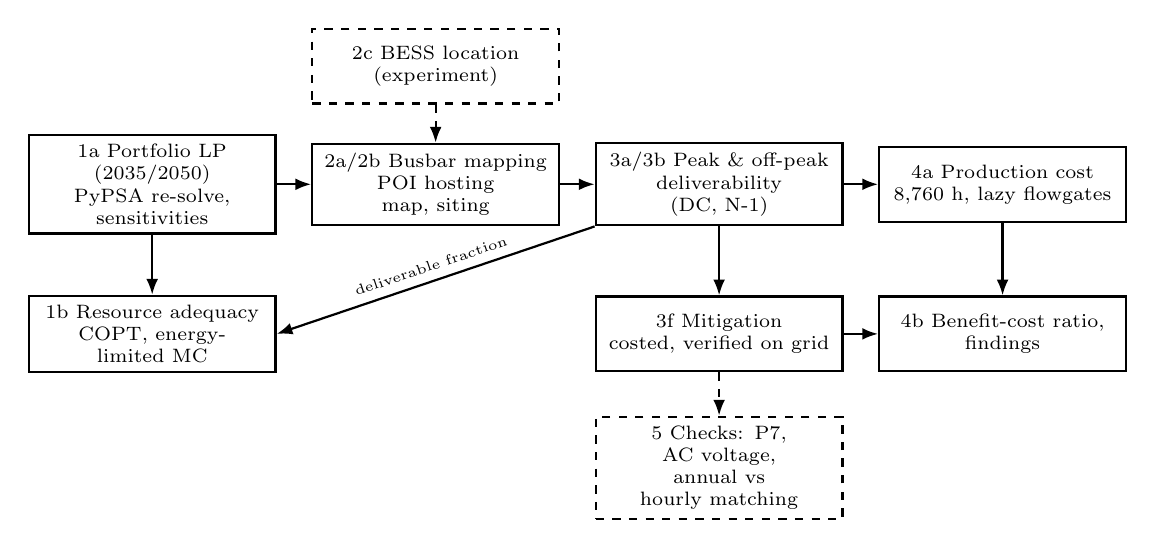
\begin{tikzpicture}[every node/.style={font=\scriptsize, align=center},
  box/.style={draw, thick, minimum width=3.0cm, minimum height=0.95cm, text width=2.9cm},
  dbox/.style={draw, thick, dashed, minimum width=3.0cm, minimum height=0.95cm, text width=2.9cm},
  ar/.style={-{Latex[length=2mm]}, thick}]
\node[box]  (p)    at (0,0)     {1a Portfolio LP (2035/2050)\\PyPSA re-solve, sensitivities};
\node[box]  (map)  at (3.6,0)   {2a/2b Busbar mapping\\POI hosting map, siting};
\node[box]  (del)  at (7.2,0)   {3a/3b Peak \& off-peak\\deliverability (DC, N-1)};
\node[box]  (pcm)  at (10.8,0)  {4a Production cost\\8,760 h, lazy flowgates};
\node[dbox] (bess) at (3.6,1.5) {2c BESS location\\(experiment)};
\node[box]  (ra)   at (0,-1.9)  {1b Resource adequacy\\COPT, energy-limited MC};
\node[box]  (mit)  at (7.2,-1.9) {3f Mitigation\\costed, verified on grid};
\node[box]  (bcr)  at (10.8,-1.9) {4b Benefit-cost ratio,\\findings};
\node[dbox] (opt)  at (7.2,-3.6) {5 Checks: P7, AC voltage,\\annual vs hourly matching};
\draw[ar] (p) -- (map); \draw[ar] (map) -- (del); \draw[ar] (del) -- (pcm); \draw[ar] (pcm) -- (bcr);
\draw[ar] (p) -- (ra); \draw[ar] (del) -- (mit); \draw[ar] (mit) -- (bcr); \draw[ar, dashed] (bess) -- (map);
\draw[ar] (del.south west) -- node[above, sloped, font=\tiny]{deliverable fraction} (ra.east);
\draw[ar, dashed] (mit) -- (opt);
\end{tikzpicture}
\caption{Study flow (solid: core assessment, after the CAISO policy-driven assessment; dashed: experiments and checks).}
\label{fig:flow}
\end{figure}

\paragraph{Data.} The hourly capacity-expansion model (one weather year, 8,760 hours, MG as one area with an import bound) and its two
saved solutions are the portfolio record. The network is the EPE 2035 planning case exported from ANAREDE (1,489 buses, 1,890 branches),
an MG-centred equivalent whose boundary buses carry \NheadroomAtwo~MW of inflows and 18,002~MW of outflows. It is an evening snapshot with
all 106 existing PV buses at 0~MW and is also used for 2050 (no 2050 network exists). Forced-outage data are NERC GADS class averages
\citep{nerc_gads_b4}; unit costs come from published EPE and ANEEL documents \citep{epe_nt047_2022,epe_nt029_2023,epe_re071_2025,aneel_bpr};
unserved energy is valued at the 2025 Custo do D\'eficit \citep{ccee2025deficit}. Optimisation uses PyPSA \citep{brown2018pypsa} with
linopy \citep{hofmann2023linopy} and HiGHS \citep{huangfu2018highs}.

% ---------------------------------------------------------------------------------------------------------------------------
\section{Portfolios (1a)}
The portfolio LP minimises the present value of incremental capital, fixed O\&M and operating cost subject to hourly balance, policy
capacity floors (PLAC-MG), resource ceilings, a monthly hydro energy budget with ramping, an import bound of 4.89~GW, and battery
state-of-charge dynamics; 2050 requires local supply without imports or gas. We rebuilt the single-year LP in PyPSA (one bus; extendable
generators and storage; custom constraints for the monthly hydro budget, cyclic ramping and the single battery converter).
The PyPSA model reproduces the saved objectives (\RS\NobjA~M and \RS\NobjB~M) and capacity mixes to within $10^{-12}$
(relative), and a re-solve of the original code under dry hydrology (\RS\NobjdryA~M and \RS\NobjdryB~M) to the same precision.
The model's 2035 stage counts capital and fixed O\&M over 2031--2050 but operating cost only over 2031--2035, so the two
objectives are not comparable; the saved portfolios are kept unchanged, since every later step depends on them.
The 2035 portfolio sits entirely on the policy floors (1.0~GW central PV, 1.04~GW distributed PV, 0.88~GW biomass, 0.30~GW small hydro);
the 2050 portfolio adds 12.9~GW central PV, 7.9~GW distributed PV, 2.0~GW wind, 0.4~GW biogas and 5.3~GW of 8-hour batteries
(Figure~\ref{fig:portfolio} and Table~\ref{tab:portfolios}). Sensitivity portfolios follow the CAISO/PJM list \citep{course_l9}: load $\pm$6\%, dry and (parametric) wet
hydrology and gas price. In 2035 they leave the portfolio unchanged; in 2050 load +6\% and dry hydrology add storage and solar.

\begin{figure}[htbp]\centering
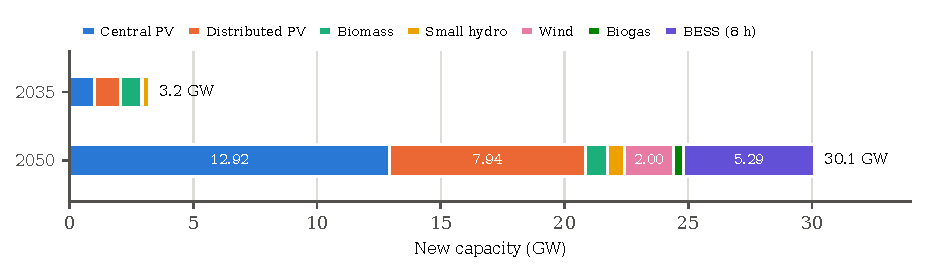
\includegraphics[width=0.92\linewidth]{figures/portfolio_mix.pdf}
\caption{New capacity of the 2035 and 2050 base portfolios by technology (LP record, reproduced in PyPSA). Battery storage is shown as power. Segments too narrow for a label: \Nportfolionarrow.}\label{fig:portfolio}
\end{figure}

\begin{table}[!htbp]
\centering
\footnotesize
\caption{Base and sensitivity portfolios (PyPSA): present-value cost, new capacity (GW) and annual energy (TWh). Sensitivities follow the CAISO/PJM list (Lectures 9--10): load $\pm$6\%, dry and wet hydrology, gas price. \enquote{Wet} is a labelled parametric +10\% monthly hydro energy (no wet-year data); curtailment is not unique in the LP (zero-cost resources). Biomass + small hydro + biogas is 1.17~GW (2035) and 1.95~GW (2050) in every case.}
\label{tab:portfolios}
\begin{adjustbox}{max width=\linewidth}
\begin{tabular}{rlrrrrrrr}
\toprule
Year & Portfolio & Cost (R\$ M) $\downarrow$ & PV & DG PV & Wind & BESS & Imports & Curtailed \\
\midrule
2035 & Base (LP record) & 15,753 & 1.00 & 1.04 & 0.00 & 0.00 & 2.29 & 1.32 \\
2050 & Base (LP record) & 20,285 & 12.92 & 7.94 & 2.00 & 5.29 & 0.00 & 15.01 \\
2035 & load +6\% & 17,734 & 1.00 & 1.04 & 0.00 & 0.00 & 5.77 & 0.12 \\
2035 & load -6\% & 15,043 & 1.00 & 1.04 & 0.00 & 0.00 & 1.05 & 3.35 \\
2035 & hydro dry & 22,651 & 1.00 & 1.04 & 0.00 & 0.00 & 14.41 & 0.26 \\
2035 & hydro wet (param.) & 15,110 & 1.00 & 1.04 & 0.00 & 0.00 & 1.16 & 3.27 \\
2035 & gas +50\% & 15,753 & 1.00 & 1.04 & 0.00 & 0.00 & 2.29 & 1.32 \\
2035 & gas -25\% & 15,753 & 1.00 & 1.04 & 0.00 & 0.00 & 2.29 & 1.32 \\
2050 & load +6\% & 24,062 & 17.41 & 7.94 & 2.00 & 6.58 & 0.00 & 16.10 \\
2050 & load -6\% & 17,054 & 10.75 & 7.94 & 2.00 & 3.36 & 0.00 & 17.57 \\
2050 & hydro dry & 27,421 & 10.75 & 16.60 & 2.00 & 8.85 & 0.00 & 8.54 \\
2050 & hydro wet (param.) & 17,469 & 10.75 & 7.94 & 2.00 & 3.74 & 0.00 & 16.60 \\
2050 & gas +50\% & 20,285 & 12.92 & 7.94 & 2.00 & 5.29 & 0.00 & 15.01 \\
2050 & gas -25\% & 20,285 & 12.92 & 7.94 & 2.00 & 5.29 & 0.00 & 15.01 \\
\bottomrule
\end{tabular}
\end{adjustbox}
\end{table}


% ---------------------------------------------------------------------------------------------------------------------------
\section{Resource adequacy (1b)}\label{sec:ra}
Adequacy is tested two ways \citep{course_l4,course_l5,course_l8}. \textbf{Method A} is the course's capacity outage probability table:
dispatchable units (reservoir hydro, gas, biogas) are convolved with GADS EFORd values (Table~\ref{tab:gads}); hydro availability in each
hour is the model's hourly upper bound scaled by the available share of installed units; profile-based resources and the firm import bound
reduce the load; batteries shave each day's net-load peaks. LOLE, LOLH and EUE follow, and ELCC values use the CAISO calibration (add or
remove perfect capacity to reach 0.1~day/yr with and without each resource class). \textbf{Method B} is a sequential Monte Carlo: two-state
Markov outage histories (GADS EFORd and mean outage duration) derate hydro, gas, biogas and batteries hour by hour, and each history is an
8,760-hour minimum-cost PyPSA dispatch with the monthly hydro budgets, ramping and storage dynamics. Unit data are not in the package:
the model's 13.38~GW of reservoir hydro is split over the 37 MG hydro-plant buses of the network in proportion to their reactive limits and
then into units of at most 250~MW (125/500~MW sensitivities). Only deliverable capacity counts \citep{course_l8}, so both methods are
repeated with every new resource scaled by the peak deliverable fraction $d=\min(1,\alpha_{HSN},\alpha_{SSN})=\Ndfrac$ for 2050
(Section~\ref{sec:deliv}).

\begin{table}[!htbp]
\centering
\small
\caption{Forced-outage data: NERC GADS Generating Unit Statistical Brochure 4, 2016--2020, all units reporting. Mapping: reservoir hydro $\to$ Hydro 30+ MW (one plant unit below 30 MW $\to$ Hydro 1--29 MW); gas $\to$ combined cycle; biogas engines $\to$ diesel; BESS $\to$ pumped storage (no battery class in GADS). Mean outage = forced-outage hours / forced outages.}
\label{tab:gads}
\begin{adjustbox}{max width=\linewidth}
\begin{tabular}{lrrrr}
\toprule
NERC GADS category & Units & Unit-years & EFORd (\%) & Mean outage (h) \\
\midrule
Hydro 30 Plus & 658 & 2,756 & 4.29 & 119 \\
Hydro 001-029 & 402 & 1,676 & 14.37 & 205 \\
Combined Cycle All Sizes & 345 & 1,420 & 3.87 & 37 \\
Gas Turbine 50 Plus & 459 & 2,059 & 9.27 & 72 \\
Diesel All Sizes & 151 & 657 & 7.92 & 35 \\
Pumped Storage All Sizes & 111 & 544 & 4.69 & 96 \\
\bottomrule
\end{tabular}
\end{adjustbox}
\end{table}

\begin{table}[!htbp]
\centering
\scriptsize
\caption{Method A (COPT convolution, capacity only). Firm gap: perfect capacity to add ($+$) or that could be removed ($-$) for LOLE = 0.1 day/yr. \enquote{Deliverable only} scales every new resource by the peak deliverable fraction $\min(1,\alpha_{HSN},\alpha_{SSN})$.}
\label{tab:copt}
\begin{adjustbox}{max width=\linewidth}
\begin{tabular}{rlrrrr}
\toprule
Year & Counting & LOLE (d/yr) $\downarrow$ & LOLH (h/yr) $\downarrow$ & EUE (MWh/yr) $\downarrow$ & Firm gap to 0.1 d/yr (MW) $\downarrow$ \\
\midrule
2035 & nameplate & 0.000 & 0.00 & 0 & -3,564 \\
2035 & nameplate, unit max 125 MW & 0.000 & 0.00 & 0 & -3,749 \\
2035 & nameplate, unit max 500 MW & 0.000 & 0.00 & 0 & -3,250 \\
2035 & nameplate, no firm imports & 112.977 & 253.00 & 64,686 & 1,329 \\
2050 & nameplate & 0.000 & 0.00 & 0 & -1,283 \\
2050 & deliverable only & 7.994 & 13.62 & 2,379 & 717 \\
2050 & nameplate, unit max 125 MW & 0.000 & 0.00 & 0 & -1,422 \\
2050 & nameplate, unit max 500 MW & 0.000 & 0.00 & 0 & -1,021 \\
\bottomrule
\end{tabular}
\end{adjustbox}
\end{table}

\begin{table}[!htbp]
\centering
\scriptsize
\caption{Method B (sequential Monte Carlo, energy-limited PyPSA dispatch, 100 outage histories per case; dry = dry-hydrology analogue). EUE in MWh/yr and \% of load; P(any): probability of any shortfall in the year. P(any shortfall) bounds LOLE from below (each year with a shortfall has $\ge$1 loss-of-load day). Firm gap: perfect capacity for P(any shortfall) $\le$ 0.1, by bisection on 0--12,000 MW to 93.75~MW resolution (each value is the upper end of its interval). \enquote{Deliverable only} scales the output of new resources by $d$ in every hour, a loose upper bound in an energy dispatch (midday output is deliverable). $^\dagger$Depends on how energy deficits are spread over hours (rotating 5\% tranches).}
\label{tab:smc}
\begin{adjustbox}{max width=\linewidth}
\begin{tabular}{rllrrrrrr}
\toprule
Year & Hydrology & Counting & No-outage EUE $\downarrow$ & EUE $\downarrow$ & EUE (\%) $\downarrow$ & P(any) $\downarrow$ & LOLE (d/yr)$^\dagger$ $\downarrow$ & Firm gap (MW) $\downarrow$ \\
\midrule
2035 & normal & nameplate & 0 & 0 & 0.000 & 0.00 & 0.0 & 0 \\
2035 & dry & nameplate & 0 & 0 & 0.000 & 0.00 & 0.0 & 0 \\
2050 & normal & nameplate & 0 & 43,988 & 0.045 & 1.00 & 28.8 & 94 \\
2050 & normal & deliverable only & 2,800,356 & 2,863,617 & 2.947 & 1.00 & 126.8 & 1,688 \\
2050 & dry & nameplate & 2,612,405 & 2,859,322 & 2.942 & 1.00 & 215.3 & 1,594 \\
2050 & dry & deliverable only & 13,768,440 & 13,969,726 & 14.374 & 1.00 & 365.0 & 3,375 \\
\bottomrule
\end{tabular}
\end{adjustbox}
\end{table}


\paragraph{Findings.} With the model's firm import bound, 2035 is comfortably adequate (no unserved energy in either method or
hydrology; Method A could remove \NpcsurplusA~MW of perfect capacity and stay at 0.1~day/yr). Without firm imports MG alone would need
\NpcgapAnameplatenofirmimports~MW more firm capacity. For 2050, Method A again reports an adequate system at nameplate, but Method B, which
sees the monthly hydro energy budgets, finds unserved energy in every simulated year (\NeueBnormalname~GWh on average,
P(any shortfall) = \NpanyBnormalname); at most \NgapBnormalname~MW of firm capacity would bring P(any shortfall) to 0.1 (the gap search resolves \Ngapres~MW). Counting only deliverable
capacity raises the Method-A gap to \NpcgapBdeliverableonly~MW, and a dry year leaves \NeueBdryname~GWh unserved (\NeuepctBdryname\% of
load) even at nameplate, needing at most \NgapBdryname~MW of firm capacity. Method B's deliverable-only case scales the new resources' output by
$d$ in every hour and so also removes midday energy that is deliverable ($\alpha=\NalphaBSonepeakdelivery$ in S1); its \NeueBnormaldel~GWh
(normal hydrology) is a loose upper bound, against \Nensbexistinggrid~GWh in the production-cost run that applies the grid hour by hour
(Section~\ref{sec:pcm}). The 2050 portfolio meets energy on average but has no reserve for
outages or drought. ELCC values (Appendix Table~\ref{tab:elcc}) show the expected pattern: new solar contributes little at the evening peak,
8-hour batteries contribute most of their nameplate.

% ---------------------------------------------------------------------------------------------------------------------------
\section{Busbar mapping and hosting capacity (2a--2c)}
The reference siting places each technology's allocation in each candidate area at the nearest eligible substation (lowest eligible
voltage on ties). A connection-cost MILP comparing a 4-area northern set with a 12-area regional set gives the POI half of
interconnection cost (Table~\ref{tab:regional}): \RS\NpoicostAL~M vs \RS\NpoicostAR~M in 2035 and \RS\NpoicostBL~M vs \RS\NpoicostBR~M in
2050. Network upgrade costs, the other half, are in Section~\ref{sec:mitigation}.

Figure~\ref{fig:poi} is the per-POI hosting map in the style of NREL's Finding~1: the injection one POI can make alone before the first
attributable violation. \Npoiabovefive{} of the \Nnpoi{} candidate stations can host at least 5~GW; the largest is \Npoitopname{}
(\Npoitop~MW). 345 and 230~kV stations host 0.3--3.3~GW.

\begin{table}[!htbp]
\centering
\small
\caption{Busbar-mapping alternatives: optimised POI connection cost (the POI half of interconnection cost; network upgrades in Section~\ref{sec:mitigation}).}
\label{tab:regional}
\begin{adjustbox}{max width=\linewidth}
\begin{tabular}{rlr}
\toprule
Year & Candidate set & POI connection cost (R\$ M) $\downarrow$ \\
\midrule
2035 & Local 4 North MG & 1,285.1 \\
2035 & Regional 12 Areas & 878.3 \\
2050 & Local 4 North MG & 5,338.2 \\
2050 & Regional 12 Areas & 4,618.8 \\
\bottomrule
\end{tabular}
\end{adjustbox}
\end{table}

\begin{figure}[htbp]\centering
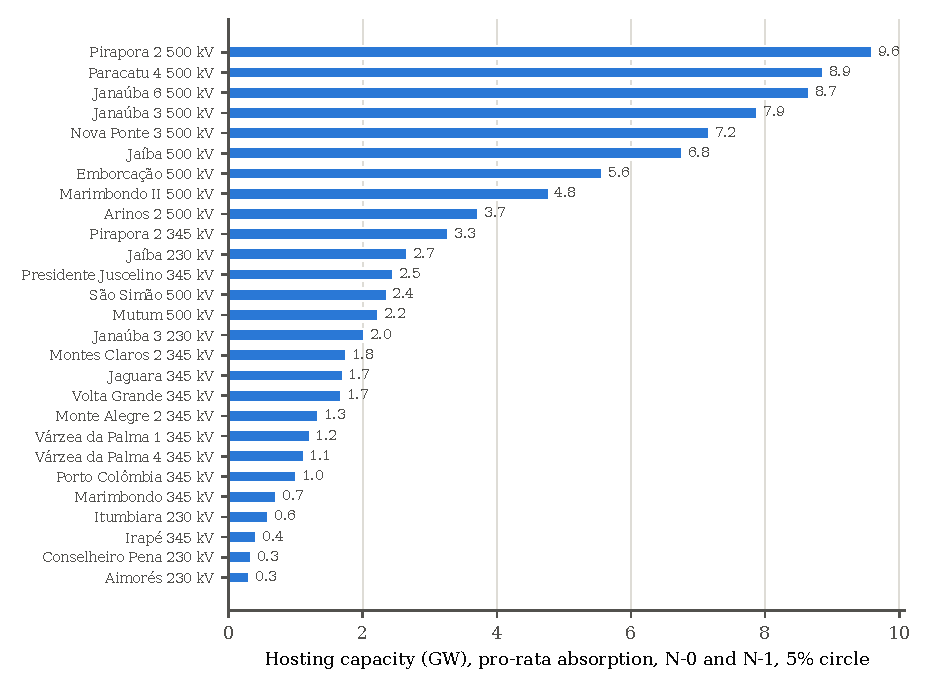
\includegraphics[width=0.86\linewidth]{figures/poi_hosting.pdf}
\caption{Per-POI hosting capacity of the 2050 candidate stations (pro-rata absorption, N-0 and N-1, 5\% circle).}\label{fig:poi}
\end{figure}

% ---------------------------------------------------------------------------------------------------------------------------
\section{Deliverability and reliability (3a--3e)}\label{sec:deliv}
\paragraph{Method.} Flows are incremental DC flows anchored on the AC solution, $f=F_{AC}+\mathrm{PTDF}\,\Delta p$, with line-outage
distribution factors for N-1 (normal ratings for N-0, emergency ratings for N-1) on \Nmonlines{} lines and \Nmontx{} transformer branches
(\Nncont{} contingencies; \Nnbridges{} radial outages skipped). The injected portfolio must be absorbed: following the CAISO convention all
other online generation is scaled down in proportion to its output (MG hydro and thermal plus the boundary inflow equivalents,
\NheadroomP~MW of headroom), with the load at the target-year level (2050 adds \NgrowthMW~MW pro rata to existing load). A facility is
attributed to the portfolio only inside the CAISO 5\% circle: some study unit has a distribution factor $\ge$5\% on it or a flow impact
$\ge$5\% of its rating \citep{caiso2018deliv,course_l11}. The one pre-existing N-1 overload of the base case is a reliability need and is
reported separately. Peak deliverability uses the model's evening hours of highest battery and non-solar output (S3) and the CAISO HSN/SSN
definitions; off-peak deliverability uses the model's midday hours of highest new output after (S1) and before (S2) curtailment
(Appendix Table~\ref{tab:factors}). $\alpha$ is the largest scaling of the joint study output that meets every attributable limit.

\paragraph{Validation.} The DC engine reproduces the earlier study's 663.31~MW and 8.62~MW results; PyPSA's PTDF, branch-outage
distribution factors and linear power flow agree with it to $\le 2\times10^{-9}$; LODF and multiple-outage factors agree with explicit
re-solves ($10^{-11}$ and $\Npgate$~MW).

\begin{table}[!htbp]
\centering
\footnotesize
\caption{Deliverability of the fixed portfolios, reference siting, main case (pro-rata absorption, target-year load, 5\% circle). $\alpha$: largest scaling of the joint study output meeting every attributable N-0/N-1 limit ($\alpha\ge1$: deliverable).}
\label{tab:deliv}
\begin{adjustbox}{max width=\linewidth}
\begin{tabular}{rlrrrrrl}
\toprule
Year & Study condition & Need MW & $\alpha$ $\uparrow$ & Groups $\downarrow$ & New viol. $\downarrow$ & Pre-ex. +MW $\downarrow$ & First binding element \\
\midrule
2035 & S1 midday (LP-used) & 1,552 & 7.48 & 0 & 0 & 0 & Marimbondo–Porto Colômbia 345 kV \\
2035 & S2 midday (pre-curt.) & 1,585 & 7.34 & 0 & 0 & 0 & Marimbondo–Porto Colômbia 345 kV \\
2035 & S3 evening (BESS) & 753 & 5.58 & 0 & 0 & 0 & Marimbondo–Porto Colômbia 345 kV \\
2035 & HSN (CAISO) & 540 & 5.89 & 0 & 0 & 0 & Marimbondo–Porto Colômbia 345 kV \\
2035 & SSN (CAISO) & 993 & 7.01 & 0 & 0 & 0 & Marimbondo–Porto Colômbia 345 kV \\
2050 & S1 midday (LP-used) & 8,177 & 1.22 & 0 & 0 & 0 & Irapé 345 kV transformer \\
2050 & S2 midday (pre-curt.) & 11,142 & 0.95 & 1 & 2 & 0 & Irapé 345 kV transformer \\
2050 & S3 evening (BESS) & 7,262 & 0.58 & 8 & 21 & 91 & Irapé 345 kV transformer \\
2050 & HSN (CAISO) & 7,073 & 0.62 & 9 & 22 & 91 & São Gonçalo do Pará 138 kV transformer \\
2050 & SSN (CAISO) & 10,092 & 0.93 & 1 & 2 & 43 & Irapé 345 kV transformer \\
\bottomrule
\end{tabular}
\end{adjustbox}
\end{table}


\paragraph{Results.} The 2035 additions are deliverable everywhere with 5.6--7.5$\times$ margin. In 2050 the midday output is
deliverable after the model's own curtailment ($\alpha=\NalphaBSonepeakdelivery$) and almost before it ($\NalphaBStwoprecurtailment$),
whereas evening delivery is not: $\alpha=\NalphaBSthreeeveningnonsolar$ (S3) and \NalphaBHSNcaiso{} (HSN), with \NupsBSthreeeveningnonsolar{}
to \NupsBHSNcaiso{} upgrade groups, mostly transformation at Ir\'ape, Montes Claros~2, Jana\'uba~3 and S\~ao Gon\c{c}alo do Par\'a. The cause
is the battery fleet: 3.7 of 5.3~GW are allocated to Montes Claros and Jana\'uba, and their full discharge flows south through northern
transformers. Placing the batteries at load buses lifts evening $\alpha$ to \NalphaBLSthreeeveningnonsolar{} (S3) and \NalphaBLHSNcaiso{}
(HSN) (Figure~\ref{fig:alpha}). The portfolio also worsens the base case's N-1 overload of the S\~ao Gon\c{c}alo do Par\'a 500/138~kV
transformation by up to \Npreworstadd~MW. Sensitivities (Appendix): the export-only convention scales every existing outflow tie in
proportion and makes the Itajub\'a~3--Cachoeira Paulista interface bind first; testing every row instead of the circle drives $\alpha$ to
zero through the pre-existing overload; the 2050 sensitivity portfolios with more storage (load +6\%, dry hydro) need 14--15 groups.

\begin{figure}[htbp]\centering
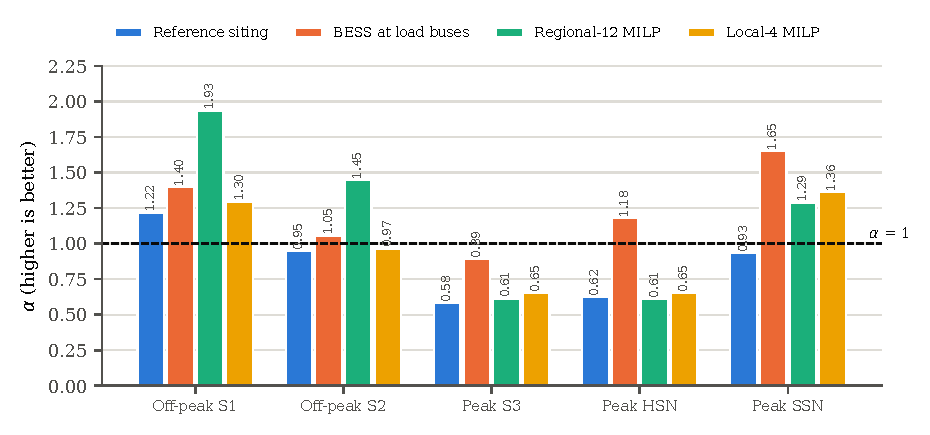
\includegraphics[width=0.92\linewidth]{figures/alpha_2050.pdf}
\caption{2050 deliverability by study condition and siting (main case). Values below the dashed line need reinforcement.}\label{fig:alpha}
\end{figure}

\paragraph{P7 and AC checks (3e, 3d).} Treating every pair of existing parallel circuits on one corridor as a common structure (\Npairs{} pairs;
conservative, tower data are not available; new circuits are on their own structures), P7 binds before P1 in the three 2050 peak cases of
the reference siting (S3, HSN and SSN; Table~\ref{tab:p7}): losing two of the three Itabira~2--Itabira~5 230~kV circuits overloads the third
($\alpha=\Npsevenminrefex$). The reinforcement plan of Section~\ref{sec:mitigation}, sized for P1, leaves this need ($\alpha=\Npsevenminrefplan$). Repeating the same procedure on
the P7 rows adds \Npremn{} new 230~kV circuits: \Npremnameone{} (\Npremkmone~km routed, \RS\Npremcapexone~M; the surviving circuit needs
+\Npremincone\%) and then \Npremnametwo{} (\RS\Npremcapextwo~M): once the first circuit is in, the next binding P7 row is the plan's new
\Npremnametwo{} circuit for the loss of both existing ones. Together they cost \RS\Npremcapex~M (\RS\Npremarr~M/yr), raise the reference-siting
capex to \RS\Npremplancapex~M and lower the full-plan BCR to \Nprembcr{}; with them every condition meets P1 and P7
($\alpha\ge\Npsevenminrefrem$). With batteries at load P7 never binds first on the existing grid, and the one-bank plan meets P1 and P7
($\alpha\ge\Npsevenminbalplan$). For the AC check, PyPSA's Newton--Raphson power flow with the network's injections reproduces the PWF flows (median error \Nacmed~MW, \Nacshare\% of branches within
2~MW + 2\%, median voltage error \Nacvmed~pu). The voltage screen (Table~\ref{tab:ac}) finds two new high-voltage buses in the 2035 off-peak
cases (S1, S2), one new low-voltage bus in the 2050 evening reference cases (S3, HSN) and, with batteries at load, a voltage rise above the
normal limit at up to 27 buses in the evening as the network unloads, a condition normally handled by reactive switching that the screen
does not model.

\begin{table}[!htbp]
\centering
\scriptsize
\caption{NERC TPL P7 check (2050), $\alpha$ by network. P1: existing grid, P1 rows only; P1+P7: existing grid with P7 rows; Plan: verified reinforcement plan of Section~\ref{sec:mitigation} (sized for P1), P1+P7; Plan + remedy: with the P7 remedy circuits (--- = none needed). Every pair of existing parallel circuits on one corridor is assumed to share a structure (conservative); new circuits are on their own structures. 2035 stays deliverable with P7 ($\alpha\ge9.1$ on P7 rows).}
\label{tab:p7}
\begin{adjustbox}{max width=\linewidth}
\begin{tabular}{llrrrrl}
\toprule
Siting & Condition & P1 $\uparrow$ & P1+P7 $\uparrow$ & Plan $\uparrow$ & Plan + remedy $\uparrow$ & Binding P7 element (existing grid) \\
\midrule
Reference & S1 midday (LP-used) & 1.22 & 1.22 & 1.34 & 1.72 & Itabira 2–Itabira 5 230 kV \\
Reference & S2 midday (pre-curt.) & 0.95 & 0.95 & 1.53 & 1.53 & Paracatu 4–Emborcação 500 kV \\
Reference & S3 evening (BESS) & 0.58 & 0.20 & 0.22 & 1.00 & Itabira 2–Itabira 5 230 kV \\
Reference & HSN (CAISO) & 0.62 & 0.21 & 0.22 & 1.00 & Itabira 2–Itabira 5 230 kV \\
Reference & SSN (CAISO) & 0.93 & 0.33 & 0.35 & 1.09 & Itabira 2–Itabira 5 230 kV \\
BESS at load & S1 midday (LP-used) & 1.40 & 1.40 & 2.18 & — & Arinos 2–Pirapora 2 500 kV \\
BESS at load & S2 midday (pre-curt.) & 1.05 & 1.05 & 1.54 & — & Paracatu 4–Emborcação 500 kV \\
BESS at load & S3 evening (BESS) & 0.89 & 0.89 & 1.46 & — & Irapé 345 kV transformer \\
BESS at load & HSN (CAISO) & 1.18 & 1.18 & 1.93 & — & Irapé 345 kV transformer \\
BESS at load & SSN (CAISO) & 1.65 & 1.65 & 1.89 & — & Paracatu 4–Emborcação 500 kV \\
\bottomrule
\end{tabular}
\end{adjustbox}
\end{table}

\begin{table}[!htbp]
\centering
\scriptsize
\caption{AC voltage screen (PyPSA Newton--Raphson, N-0, MG buses $\ge$230 kV, bus-specific normal limits of the PWF). The base case already has 5 buses above their limit. Generator reactive limits are not enforced.}
\label{tab:ac}
\begin{adjustbox}{max width=\linewidth}
\begin{tabular}{rllrrrrrl}
\toprule
Year & Siting & Condition & $V_{min}$ (pu) & $V_{max}$ (pu) & New low $\downarrow$ & New high $\downarrow$ & Min. margin (pu) $\uparrow$ & Tightest bus \\
\midrule
2035 & Reference & S1 midday (LP-used) & 0.878 & 1.091 & 0 & 2 & -0.006 & Itabira 5 230 kV \\
2035 & Reference & S2 midday (pre-curt.) & 0.878 & 1.091 & 0 & 2 & -0.006 & Itabira 5 230 kV \\
2035 & Reference & S3 evening (BESS) & 0.878 & 1.089 & 0 & 0 & -0.005 & Itabira 5 230 kV \\
2035 & Reference & HSN (CAISO) & 0.878 & 1.089 & 0 & 0 & -0.004 & Itabira 5 230 kV \\
2035 & Reference & SSN (CAISO) & 0.878 & 1.089 & 0 & 0 & -0.005 & Itabira 5 230 kV \\
2050 & BESS at load & S1 midday (LP-used) & 0.879 & 1.081 & 0 & 0 & 0.000 & Santos Dumont 2 345 kV \\
2050 & BESS at load & S2 midday (pre-curt.) & 0.879 & 1.079 & 0 & 0 & 0.001 & Santos Dumont 2 345 kV \\
2050 & BESS at load & S3 evening (BESS) & 0.879 & 1.100 & 0 & 26 & -0.015 & Itabira 5 230 kV \\
2050 & BESS at load & HSN (CAISO) & 0.879 & 1.101 & 0 & 27 & -0.015 & Itabira 5 230 kV \\
2050 & BESS at load & SSN (CAISO) & 0.879 & 1.085 & 0 & 0 & -0.003 & Santos Dumont 2 345 kV \\
2050 & Reference & S1 midday (LP-used) & 0.879 & 1.078 & 0 & 0 & 0.003 & Santos Dumont 2 345 kV \\
2050 & Reference & S2 midday (pre-curt.) & 0.879 & 1.078 & 0 & 0 & 0.003 & Santos Dumont 2 345 kV \\
2050 & Reference & S3 evening (BESS) & 0.879 & 1.073 & 1 & 0 & -0.007 & CVERED 345 kV \\
2050 & Reference & HSN (CAISO) & 0.879 & 1.073 & 1 & 0 & -0.002 & CVERED 345 kV \\
2050 & Reference & SSN (CAISO) & 0.879 & 1.075 & 0 & 0 & 0.008 & Aurora 3 230 kV \\
\bottomrule
\end{tabular}
\end{adjustbox}
\end{table}


\paragraph{Does a constraint subset represent the full system?} The production-cost run needs a manageable set of flow constraints. Rows
loaded $\ge$90\% at full study output in any of the \Nsubsetcases{} cases form a subset of \Nsubsetpairs{} rows (\Nsubsetpct\% of
\Nsubsetrowsfull), \Nsubsetelements{} elements in \Nsubsetgroups{} groups. Because removing constraints can only make a problem more
optimistic, a solution that satisfies all omitted rows is optimal for the full problem; and any row that binds at $\alpha<1$ is loaded
$\ge$100\% at full output, so it is in the subset. Empirically $\alpha$ is identical in \Nsubsetinsampleexactalphaltone{} of
\Nsubsetcasesalphaltone{} in-sample cases with $\alpha<1$ and in \Nsubsetoutofsampleexactalphaltone{} of
\Nsubsetoutofsamplecasesalphaltone{} out-of-sample cases (subset drawn from the reference siting only). The production-cost run therefore
adds flowgates lazily and re-checks every hour on all rows (Section~\ref{sec:pcm}).

% ---------------------------------------------------------------------------------------------------------------------------
\section{Mitigation and battery siting (3f, 2c)}\label{sec:mitigation}
For each attributable group the alternatives follow the PG\&E cluster-study structure \citep{course_l12}: status quo; limiting-element
removal or re-rating; reconductoring; transformer addition or new circuit; storage (here, siting the planned batteries at load); grid-enhancing
technologies such as dynamic line rating \citep{course_l6}; and remedial action schemes. Costed alternatives use published unit costs
(Appendix Table~\ref{tab:unitcosts}): EPE/ONS and EPE transformer and bay costs at ANEEL reference prices, EPE line costs, and EPE's
finding that reconductoring costs 65--108.5\% of a new circuit. Sizing assumes identical parallel elements share flow equally. The plan is
then verified on a network that actually contains the new elements (PTDF and LODF rebuilt, base flows re-anchored): every study condition is
deliverable on the first pass (smallest $\alpha=\Nveralphamin$).

\begin{table}[!htbp]
\centering
\footnotesize
\caption{Attributable reinforcement plan (2050, main case), verified on a network that contains the new elements. Need: largest required increase over the study conditions. Non-wires candidate: line need $\le$10\%, where re-rating, limiting-element removal or dynamic line rating may suffice (not costable with the data). Existing: parallel elements in the group.}
\label{tab:plan}
\begin{adjustbox}{max width=\linewidth}
\begin{tabular}{llrrlrrl}
\toprule
Siting & Upgrade group & Need (\%) & Existing & Least-cost alternative & Elements & Capex (R\$ M) $\downarrow$ & Non-wires \\
\midrule
Reference & Ipatinga 1–Mesquita 230 kV & 3.9 & 2 & new circuit & 1 & 24.7 & yes \\
Reference & Ipatinga 1–Timóteo 2 230 kV & 4.3 & 1 & reconductor (HTLS) & 1 & 32.3 & yes \\
Reference & Jaguara–Volta Grande 345 kV & 3.1 & 1 & reconductor (HTLS) & 1 & 231.0 & yes \\
Reference & Montes Claros 2–Várzea da Palma 345 kV & 6.0 & 1 & reconductor (HTLS) & 1 & 383.4 & yes \\
Reference & Volta Grande–L.C. Barreto 345 kV & 0.4 & 1 & reconductor (HTLS) & 1 & 311.4 & yes \\
Reference & Irapé 345/230 kV transf. & 68.5 & 2 & add bank(s) & 2 & 94.1 &  \\
Reference & Janaúba 3 500/230 kV transf. & 13.1 & 5 & add bank(s) & 1 & 57.6 &  \\
Reference & Montes Claros 2 345/138 kV transf. & 23.3 & 2 & add bank(s) & 1 & 60.7 &  \\
Reference & São Gonçalo do Pará 500/138 kV transf. & 7.5 & 3 & add bank(s) & 1 & 54.4 &  \\
BESS at load & Irapé 345/230 kV transf. & 9.4 & 2 & add bank(s) & 1 & 47.0 &  \\
\bottomrule
\end{tabular}
\end{adjustbox}
\end{table}


The reference-siting plan has \NgroupsR{} groups. Its costed total is \RS\NcapexR~M (\RS\NcapexlowR--\NcapexhighR~M across the
reconductoring range); five line needs are below 10\% and are candidates for re-rating or dynamic rating, without which the plan is the four
transformer additions, \RS\NcapexexclR~M. With batteries at load the plan is one Ir\'ape bank, \RS\NcapexL~M. The pre-existing
S\~ao Gon\c{c}alo do Par\'a overload (\Nprebase~MW in the base case) is a reliability need requiring one bank (\RS\Nprecapexbase~M); the
portfolio's \Npreadd~MW raises it to \Nprebanks{} banks, an attributable increment of \RS\Nprecapexinc~M (possibly the same bank as the
plan's S\~ao Gon\c{c}alo do Par\'a addition).

% ---------------------------------------------------------------------------------------------------------------------------
\section{Economic assessment (4a, 4b)}\label{sec:pcm}
\paragraph{Method.} The fixed portfolio is dispatched hour by hour in PyPSA with the model's costs and limits plus DC flowgates on the main
grid \citep{course_l9}. Hourly changes relative to the network snapshot are injected on their buses: the snapshot corresponds to the 2035
model hour with the same MG load (10,731~MW) and hydro output (5,132~MW); load, existing distributed generation and unserved energy go to
load buses pro rata, reservoir hydro to the hydro-plant buses, imports to the boundary inflow equivalents, existing PV equally to the PV buses,
thermal to the thermal buses, and new resources and batteries to their POIs, so the changes balance exactly. Months are solved separately
with the monthly hydro budgets and month-boundary battery states taken from the annual unconstrained dispatch; flowgates are added lazily
until no N-0 or N-1 row is violated in any hour. Annual system cost is production cost plus unserved energy at \RS8,327.76/MWh
\citep{ccee2025deficit} plus unused zero-cost energy (curtailment of the profile-based resources as defined in the model, and unused hydro budget) at the 2025
SE marginal cost, \RS209.47/MWh (the model's import price). Congestion curtailment is the unused zero-cost energy above the same year's run
without network limits, as a share of the available profile-based and hydro energy (the split between the two is not unique); we
screen it against a 5\% threshold (a study choice).
Without flowgates the monthly runs reproduce the annual dispatch (no unserved energy; same imports and production cost).

\begin{table}[!htbp]
\centering
\footnotesize
\caption{Network-constrained 8,760-h production cost (PyPSA, monthly, lazy flowgates on all N-0/N-1 rows). System cost = production + unserved energy at R\$ 8,327.76/MWh + unused renewable energy (VRE curtailment and unused hydro budget) at R\$ 209.47/MWh.}
\label{tab:pcm}
\begin{adjustbox}{max width=\linewidth}
\begin{tabular}{lrrrrrr}
\toprule
Scenario & Production $\downarrow$ & Unserved GWh $\downarrow$ & Unused RE TWh $\downarrow$ & System cost $\downarrow$ & Congestion $\downarrow$ & Rows \\
\midrule
2035, no network limits & 480.2 & 0.0 & 1.47 & 787 & 0 & 0 \\
2035, existing grid & 480.2 & 0.0 & 1.47 & 787 & 0 & 2 \\
2050, no network limits & 44.6 & 0.0 & 17.29 & 3,666 & 0 & 0 \\
2050, existing grid & 48.3 & 689.5 & 17.64 & 9,486 & 5,820 & 679 \\
2050, grid + plan & 46.6 & 5.9 & 17.29 & 3,718 & 52 & 401 \\
2050 BESS at load, existing grid & 45.2 & 78.3 & 17.36 & 4,333 & 667 & 319 \\
2050 BESS at load, grid + plan & 44.7 & 46.7 & 17.33 & 4,064 & 399 & 298 \\
\bottomrule
\end{tabular}
\end{adjustbox}
\par\vspace{2pt}\begin{minipage}{0.95\linewidth}\footnotesize Costs in R\$ M/yr; Rows: flowgate rows added by the lazy check.\end{minipage}
\end{table}


\paragraph{Results.} In 2035 the network constrains only \Nrowsaexistinggrid{} rows briefly and adds no congestion cost
(\RS\Ncongaexistinggrid~M/yr). In 2050 the existing grid sheds \Nensbexistinggrid~GWh of load (\Nenspctbexistinggrid\%) in every month,
a congestion cost of \RS\Ncongbexistinggrid~M/yr that is almost entirely unserved energy (Figure~\ref{fig:pcm}); without network limits
the same dispatch serves all load. The reinforcement plan reduces unserved energy to \Nensbwithplan~GWh, all in \Nbudgetminmonth, the month with the
smallest hydro energy budget (\Nbudgetmin~GWh against \Nbudgetothermin--\Nbudgetothermax~GWh in the other months), and its benefit-cost ratio is \NbcrRfull{} for the full costed plan and \NbcrRexcl{} if small line needs are met by
non-wires means (Table~\ref{tab:bcr}); because the benefit is mostly avoided unserved energy, it stays far above one in every valuation
sensitivity (minimum \NbcrRmin). Siting the batteries at load is worth \RS\Nbenreloc~M/yr before any grid investment: unserved energy falls
to \Nensbbessatloadexistinggrid~GWh, again only in \Nbudgetminmonth. Its one-bank plan leaves \Nensbbessatloadwithplan~GWh in
\Nbudgetminmonth; the flowgates that the lazy check adds concentrate on \Nfgbalplanone{} (\Nfgbalplanrowsone{} rows), \Nfgbalplantwo{}
(\Nfgbalplanrowstwo) and \Nfgbalplanthree{} (\Nfgbalplanrowsthree). Apart from the pre-existing S\~ao Gon\c{c}alo do Par\'a overload, the
study-condition screen did not flag these elements; they are candidates for an economic-driven addition. The energy-tight month, not the study hours, sets the residual
need, which is why the production-cost run is part of the assessment.

\paragraph{What drives curtailment?} Not the grid. Without any network limit, \Nunusedbcopperplate~TWh of zero-cost energy
(\Nunusedpctbcopperplate\% of the available profile-based and hydro energy) goes unused in 2050 because the hourly local-balance rule
allows no exports; the existing grid adds congestion curtailment of only \Ncongcurtpctbexistinggrid\% (\Ncongcurtpctbwithplan\% with the plan), well below
the 5\% screen. Unlike NREL's Oregon finding that congestion drives curtailment \citep{nrel2021oregon}, the grid's cost here is
unserved load, not lost energy, and the curtailed energy is what an export option would sell (next paragraph).

\begin{figure}[htbp]\centering
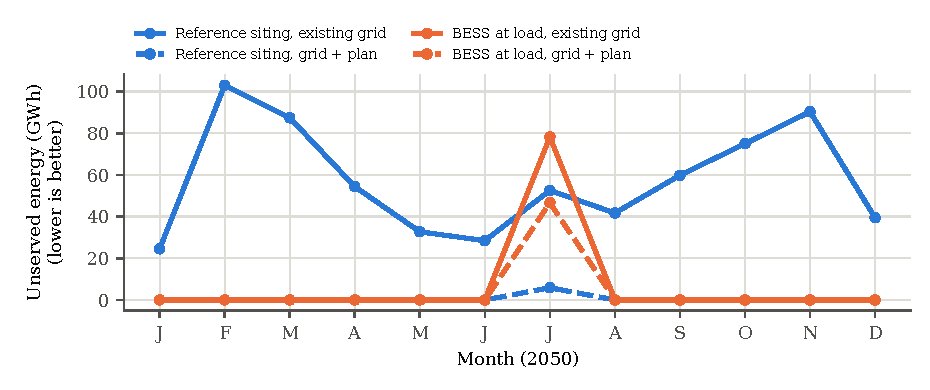
\includegraphics[width=0.92\linewidth]{figures/pcm_ens.pdf}
\caption{Monthly unserved energy in the 2050 network-constrained production-cost runs.}\label{fig:pcm}
\end{figure}
\begin{table}[!htbp]
\centering
\footnotesize
\caption{Benefit-cost ratios (annual benefit / annual revenue requirement at CRF(8\%, 30 yr) + 1.5\% O\&M). BCR $>$ 1 justifies the measure (CAISO/PJM economic criterion). Valuing unused renewable energy $\pm$50\% changes the BCRs by at most 0.9\%.}
\label{tab:bcr}
\begin{adjustbox}{max width=\linewidth}
\begin{tabular}{llrrrrr}
\toprule
Measure & Valuation & Benefit (R\$ M/yr) $\uparrow$ & Cost, full plan (R\$ M/yr) & BCR $\uparrow$ & Cost, excl. small needs & BCR $\uparrow$ \\
\midrule
Plan, reference siting & base & 5,768 & 129.7 & 44.5 & 27.7 & 208.3 \\
Plan, BESS at load & base & 268 & 4.9 & 55.0 & 4.9 & 55.0 \\
Plan, reference siting & VOLL -50\% & 2,922 & 129.7 & 22.5 & 27.7 & 105.5 \\
Plan, BESS at load & VOLL -50\% & 137 & 4.9 & 28.0 & 4.9 & 28.0 \\
Plan, reference siting & VOLL +50\% & 8,615 & 129.7 & 66.4 & 27.7 & 311.0 \\
Plan, BESS at load & VOLL +50\% & 400 & 4.9 & 81.9 & 4.9 & 81.9 \\
\bottomrule
\end{tabular}
\end{adjustbox}
\end{table}


\paragraph{Hourly or annual matching.} The 2050 requirement is hourly local balance. Allowing exports alone lowers cost by
\NmatchabsHone\% (\NmatchHexports~TWh exported); annual matching (imports allowed hour by hour, annual imports no greater than exports) lowers it
by \NmatchabsAone\% and removes the need for batteries, wind and biogas (Table~\ref{tab:matching}), in line with the course's 24/7 case
\citep{course_contracting}. That alternative relies on \NmatchAexports~TWh/yr of exports, which the export interface results above would
have to accommodate.
\begin{table}[!htbp]
\centering
\scriptsize
\caption{Hourly versus annual clean matching in 2050 (capacities in GW; gas is zero in every case).}
\label{tab:matching}
\begin{adjustbox}{max width=\linewidth}
\begin{tabular}{lrrrrrrr}
\toprule
2050 definition & Cost (R\$ M PV) $\downarrow$ & vs H0 (\%) $\downarrow$ & Central PV & Wind & BESS & Imports (TWh) & Exports (TWh) \\
\midrule
H0 hourly local balance (LP) & 20,285 & 0.0 & 12.92 & 2.00 & 5.29 & 0.0 & 0.0 \\
H1 hourly balance, exports allowed & 17,557 & -13.4 & 14.11 & 2.00 & 4.83 & 0.0 & 16.0 \\
A1 annual matching (net annual exporter) & 10,415 & -48.7 & 10.75 & 0.00 & 0.00 & 12.0 & 16.6 \\
\bottomrule
\end{tabular}
\end{adjustbox}
\end{table}


% ---------------------------------------------------------------------------------------------------------------------------
\section{Findings}
\begin{enumerate}\itemsep2pt
\item \textbf{2035: no major grid improvement is needed.} The policy portfolio is deliverable in every study condition with 5.6--7.5$\times$
margin, adds no congestion cost, and is adequate under the model's import assumption.
\item \textbf{2050 midday solar is deliverable; 2050 evening storage discharge is not.} Midday $\alpha=\NalphaBSonepeakdelivery$; evening
$\alpha=\NalphaBSthreeeveningnonsolar$--\NalphaBHSNcaiso{} because 3.7~GW of batteries sit in the north.
\item \textbf{Battery siting is the cheapest fix.} At load buses the evening need falls to one transformer bank (\RS\NcapexL~M) and the
system cost falls by \RS\Nbenreloc~M/yr.
\item \textbf{If batteries stay in the north, the attributable plan is justified.} \NgroupsR{} groups, \RS\NcapexexclR--\NcapexR~M,
BCR \NbcrRfull--\NbcrRexcl. If existing parallel circuits share towers (P7), \Npremn{} more 230~kV circuits (\RS\Npremcapex~M) are
needed and the full-plan BCR is \Nprembcr.
\item \textbf{2050 adequacy is energy-limited.} A capacity-only COPT finds no shortfall; the energy-limited simulation finds shortfalls
in every simulated year and \NeueBdryname~GWh in a dry year, needing up to \NgapBnormalname~MW (normal) and \NgapBdryname~MW (dry) of firm capacity.
\item \textbf{Curtailment comes from the hourly local-balance rule, not from congestion.} Even without network limits
\Nunusedbcopperplate~TWh (\Nunusedpctbcopperplate\%) of 2050 zero-cost energy goes unused; congestion adds \Ncongcurtpctbexistinggrid\%
(below the 5\% screen).
\item \textbf{The definition of fossil-free matters.} Annual instead of hourly matching lowers 2050 cost by \NmatchabsAone\%, if exports
can be delivered.
\end{enumerate}

\paragraph{Limitations.} One network snapshot (evening) and one weather year; the 2050 network is the 2035 topology; DC flows except for the N-0 AC voltage screen, which covers the existing grid only and does not enforce generator reactive
limits; hydro unit sizes are a proxy; reconductoring is modelled as a rating increase with unchanged
impedance and new circuits and banks as added parallel elements; P7 assumes that existing parallel circuits share structures; the
production-cost benefits are computed for the P1 plan and held at their 2050 value over the asset life.

\bibliographystyle{plainnat}
\bibliography{refs}

\appendix
\section{Supplementary tables}
\begin{table}[!htbp]
\centering
\scriptsize
\caption{Study output levels (fraction of new nameplate). S1–S3: mean of the top 1\% LP hours; HSN/SSN: CAISO exceedance definitions.}
\label{tab:factors}
\begin{adjustbox}{max width=\linewidth}
\begin{tabular}{rlrrrrr}
\toprule
Year & Technology & Off-peak S1 & Off-peak S2 & Peak S3 & Peak HSN & Peak SSN \\
\midrule
2035 & bess & 0.00 & 0.00 & 0.00 & 1.00 & 0.50 \\
2035 & bio & 0.33 & 0.34 & 0.46 & 0.43 & 0.36 \\
2035 & biogas & 0.00 & 0.00 & 0.00 & 0.70 & 0.70 \\
2035 & small hydro & 0.36 & 0.36 & 0.33 & 0.54 & 0.43 \\
2035 & solar central & 0.58 & 0.59 & 0.14 & 0.00 & 0.36 \\
2035 & solar distributed & 0.55 & 0.56 & 0.11 & 0.00 & 0.18 \\
2035 & wind site & 0.00 & 0.00 & 0.00 & 0.37 & 0.24 \\
2050 & bess & 0.11 & 0.11 & 1.00 & 1.00 & 0.50 \\
2050 & bio & 0.16 & 0.20 & 0.45 & 0.43 & 0.36 \\
2050 & biogas & 0.09 & 0.09 & 0.58 & 0.70 & 0.70 \\
2050 & small hydro & 0.35 & 0.46 & 0.34 & 0.54 & 0.43 \\
2050 & solar central & 0.31 & 0.44 & 0.01 & 0.00 & 0.36 \\
2050 & solar distributed & 0.31 & 0.43 & 0.00 & 0.00 & 0.18 \\
2050 & wind site & 0.32 & 0.42 & 0.49 & 0.37 & 0.24 \\
\bottomrule
\end{tabular}
\end{adjustbox}
\end{table}

\begin{table}[!htbp]
\centering
\scriptsize
\caption{Sensitivity of $\alpha$ $\uparrow$ to the absorption convention (reference siting, 5\% circle). For 2050 the main case includes target-year load growth; \enquote{2035 load} omits it.}
\label{tab:absorption}
\begin{adjustbox}{max width=\linewidth}
\begin{tabular}{rlrrrrrr}
\toprule
Year & Condition & Pro rata & A1 MG only & A2 inflows & B export & Pro rata, 2035 load & B, 2035 load \\
\midrule
2035 & Off-peak S1 (midday, LP-used) & 7.48 & 3.41 & 7.14 & 4.96 & — & — \\
2035 & Off-peak S2 (midday, pre-curtailment) & 7.34 & 3.34 & 7.00 & 4.86 & — & — \\
2035 & Peak S3 (evening, BESS) & 5.58 & 6.02 & 5.49 & 5.11 & — & — \\
2035 & Peak HSN (CAISO) & 5.89 & 6.23 & 5.81 & 5.50 & — & — \\
2035 & Peak SSN (CAISO) & 7.01 & 5.23 & 6.81 & 6.08 & — & — \\
2050 & Off-peak S1 (midday, LP-used) & 1.22 & 0.68 & 1.13 & 1.24 & 1.24 & 0.91 \\
2050 & Off-peak S2 (midday, pre-curtailment) & 0.95 & 0.46 & 0.87 & 0.85 & 0.96 & 0.67 \\
2050 & Peak S3 (evening, BESS) & 0.58 & 0.45 & 0.56 & 0.59 & 0.59 & 0.59 \\
2050 & Peak HSN (CAISO) & 0.62 & 0.45 & 0.63 & 0.66 & 0.66 & 0.67 \\
2050 & Peak SSN (CAISO) & 0.93 & 0.46 & 0.87 & 0.95 & 0.95 & 0.76 \\
\bottomrule
\end{tabular}
\end{adjustbox}
\end{table}

\begin{table}[!htbp]
\centering
\scriptsize
\caption{Sensitivity of $\alpha$ $\uparrow$ to the attribution rule. \enquote{Every row tested} also forbids any worsening of the one pre-existing overload, which drives $\alpha$ to zero; the cap variant raises only the highest-impact circle units (a bound).}
\label{tab:rule}
\begin{adjustbox}{max width=\linewidth}
\begin{tabular}{rlrrr}
\toprule
Year & Condition & Every row tested & 5\% circle (main) & Circle + 20 unit / 1,500 MW cap \\
\midrule
2035 & Off-peak S1 (midday, LP-used) & 7.48 & 7.48 & 7.62 \\
2035 & Off-peak S2 (midday, pre-curtailment) & 7.34 & 7.34 & 7.48 \\
2035 & Peak S3 (evening, BESS) & 5.58 & 5.58 & 5.60 \\
2035 & Peak HSN (CAISO) & 0.00 & 5.89 & 5.88 \\
2035 & Peak SSN (CAISO) & 7.01 & 7.01 & 7.03 \\
2050 & Off-peak S1 (midday, LP-used) & 0.00 & 1.22 & 1.16 \\
2050 & Off-peak S2 (midday, pre-curtailment) & 0.95 & 0.95 & 0.89 \\
2050 & Peak S3 (evening, BESS) & 0.00 & 0.58 & 0.85 \\
2050 & Peak HSN (CAISO) & 0.00 & 0.62 & 1.11 \\
2050 & Peak SSN (CAISO) & 0.00 & 0.93 & 0.89 \\
\bottomrule
\end{tabular}
\end{adjustbox}
\end{table}

\begin{table}[!htbp]
\centering
\small
\caption{Sensitivity of 2050 $\alpha$ $\uparrow$ to siting (main case).}
\label{tab:siting}
\begin{adjustbox}{max width=\linewidth}
\begin{tabular}{lrrrr}
\toprule
Condition (2050) & Reference & Reference, BESS at load & Regional-12 MILP & Local-4 MILP \\
\midrule
Off-peak S1 (midday, LP-used) & 1.22 & 1.40 & 1.93 & 1.30 \\
Off-peak S2 (midday, pre-curtailment) & 0.95 & 1.05 & 1.45 & 0.97 \\
Peak S3 (evening, BESS) & 0.58 & 0.89 & 0.61 & 0.65 \\
Peak HSN (CAISO) & 0.62 & 1.18 & 0.61 & 0.65 \\
Peak SSN (CAISO) & 0.93 & 1.65 & 1.29 & 1.36 \\
\bottomrule
\end{tabular}
\end{adjustbox}
\end{table}

\begin{table}[!htbp]
\centering
\small
\caption{Midday sensitivity with existing central PV (split equally over the 106 UFV buses) and existing DG added.}
\label{tab:existingpv}
\begin{adjustbox}{max width=\linewidth}
\begin{tabular}{rlrrl}
\toprule
Year & Absorption & Need (MW) & $\alpha$ $\uparrow$ & Status \\
\midrule
2035 & Pro rata & 9,666 & 2.39 & deliverable \\
2035 & A1 MG only & 9,666 & 0.51 & energy-limited \\
2035 & A2 inflows & 9,666 & 2.26 & deliverable \\
2035 & B export & 9,666 & 0.77 & needs upgrades \\
2050 & Pro rata & 12,743 & 1.20 & deliverable \\
2050 & A1 MG only & 12,743 & 0.42 & energy-limited \\
2050 & A2 inflows & 12,743 & 1.06 & deliverable \\
2050 & B export & 12,743 & 0.71 & needs upgrades \\
\bottomrule
\end{tabular}
\end{adjustbox}
\end{table}

\begin{table}[!htbp]
\centering
\scriptsize
\caption{Peak deliverability of the 2050 sensitivity portfolios (reference siting by allocation weights, main case). The 2035 sensitivity portfolios equal the base portfolio (policy floors bind) and stay deliverable ($\alpha\ge3.45$).}
\label{tab:sensdeliv}
\begin{adjustbox}{max width=\linewidth}
\begin{tabular}{llrrr}
\toprule
Sensitivity portfolio (2050) & Cond. & Need (MW) & $\alpha$ $\uparrow$ & Upgrade groups $\downarrow$ \\
\midrule
load +6\% & HSN & 8,364 & 0.46 & 15 \\
load +6\% & SSN & 12,352 & 0.74 & 5 \\
load -6\% & HSN & 5,140 & 0.83 & 1 \\
load -6\% & SSN & 8,346 & 1.15 & 0 \\
hydro dry & HSN & 10,634 & 0.47 & 14 \\
hydro dry & SSN & 12,648 & 0.75 & 3 \\
hydro wet (param.) & HSN & 5,525 & 0.63 & 4 \\
hydro wet (param.) & SSN & 8,538 & 1.10 & 0 \\
gas +50\% & HSN & 7,073 & 0.62 & 9 \\
gas +50\% & SSN & 10,092 & 0.93 & 1 \\
gas -25\% & HSN & 7,073 & 0.62 & 9 \\
gas -25\% & SSN & 10,092 & 0.93 & 1 \\
\bottomrule
\end{tabular}
\end{adjustbox}
\end{table}

\begin{table}[!htbp]
\centering
\scriptsize
\caption{Effective load-carrying capability by the CAISO calibration (Lecture 11, method A).}
\label{tab:elcc}
\begin{adjustbox}{max width=\linewidth}
\begin{tabular}{rllrrr}
\toprule
Year & Counting & Resource class & Nameplate (MW) & ELCC (MW) $\uparrow$ & ELCC (\% of nameplate) $\uparrow$ \\
\midrule
2035 & nameplate & new solar (central + DG) & 2,044 & 1 & 0.0 \\
2035 & nameplate & new biomass + small hydro & 1,173 & 305 & 26.0 \\
2035 & nameplate & all new resources & 3,217 & 306 & 9.5 \\
2050 & nameplate & new solar (central + DG) & 20,862 & 3,304 & 15.8 \\
2050 & nameplate & new BESS & 5,290 & 4,734 & 89.5 \\
2050 & nameplate & new wind & 2,000 & 391 & 19.5 \\
2050 & nameplate & new biomass + small hydro & 1,548 & 523 & 33.8 \\
2050 & nameplate & new biogas & 400 & 256 & 64.1 \\
2050 & nameplate & all new resources & 30,101 & 5,786 & 19.2 \\
2050 & deliverable only & new solar (central + DG) & 20,862 & 928 & 4.4 \\
2050 & deliverable only & new BESS & 5,290 & 3,082 & 58.2 \\
2050 & deliverable only & new wind & 2,000 & 215 & 10.7 \\
2050 & deliverable only & new biomass + small hydro & 1,548 & 323 & 20.9 \\
2050 & deliverable only & new biogas & 400 & 156 & 38.9 \\
2050 & deliverable only & all new resources & 30,101 & 3,786 & 12.6 \\
\bottomrule
\end{tabular}
\end{adjustbox}
\end{table}

\begin{table}[!htbp]
\centering
\scriptsize
\caption{Unit costs used for the costed alternatives (published EPE/ANEEL values; price bases differ and are not indexed).}
\label{tab:unitcosts}
\begin{adjustbox}{max width=\linewidth}
\begin{tabular}{>{\raggedright\arraybackslash}p{3.6cm}>{\raggedright\arraybackslash}p{1.7cm}r>{\raggedright\arraybackslash}p{5.4cm}>{\raggedright\arraybackslash}p{2.6cm}}
\toprule
Item & Unit & Value (R\$ M or ratio) & Source & Price basis \\
\midrule
ATF single-phase unit 500/345 kV 500 MVA & per unit (500 MVA) & 23.875 & EPE/ONS EPE-DEE-NT-047-2022 (RT-ONS DPL 0355/2022) Avaliação dos benefícios sistêmicos do TR 500/345 kV na SE UTE GNA & ANEEL BPR (as used in the note) \\
ATF single-phase unit 500/230 kV 100 MVA & per unit (100 MVA) & 10.975 & EPE-DEE-RE-071-2025-rev0 & ANEEL Ref. 2025/0123 \\
ATF single-phase unit 345/138 kV 100 MVA & per unit (100 MVA) & 11.232 & EPE-DEE-NT-029-2023-rev0 Ampliação da SE Campinas 345/138 kV & ANEEL BPR base March 2023 \\
CT transformer connection bay 500 kV (DJM) & per bay & 15.044 & EPE-DEE-NT-047-2022 & ANEEL BPR (as used in the note) \\
CT transformer connection bay 345 kV (DJM) & per bay & 12.106 & EPE-DEE-NT-047-2022 & ANEEL BPR (as used in the note) \\
CT transformer connection bay 230 kV (BD4) & per bay & 9.668 & EPE-DEE-RE-071-2025-rev0 & ANEEL Ref. 2025/0123 \\
CT transformer connection bay 138 kV (BD4) & per bay & 6.430 & EPE-DEE-NT-029-2023-rev0 & ANEEL BPR base March 2023 \\
New line 230 kV & per km & 1.104 & EPE-DEE-RE-071-2025-rev0 (inputs/cost\_assumptions.json) & EPE 2025 (project cost file) \\
New line 345 kV single circuit 4x954 MCM & per km & 2.388 & EPE-DEE-NT-047-2022 & ANEEL BPR (as used in the note) \\
New line 500 kV & per km & 2.469 & EPE-DEE-RE-071-2025-rev0 (inputs/cost\_assumptions.json) & EPE 2025 (project cost file) \\
Line entry bay 230 kV & per bay & 10.501 & EPE-DEE-RE-071-2025-rev0 (inputs/cost\_assumptions.json) & EPE 2025 (project cost file) \\
Line entry bay 345 kV (DJM) & per bay & 10.518 & EPE-DEE-NT-047-2022 & ANEEL BPR (as used in the note) \\
Line entry bay 500 kV & per bay & 13.398 & EPE-DEE-RE-071-2025-rev0 (inputs/cost\_assumptions.json) & EPE 2025 (project cost file) \\
Reconductoring vs new line (total cost ratio) & ratio & 0.650 & EPE-DEE-RE-071-2025-rev0 & ANEEL Ref. 2025/0123 \\
Reconductoring vs new line (total cost ratio) & ratio & 1.085 & EPE-DEE-RE-071-2025-rev0 & ANEEL Ref. 2025/0123 \\
\bottomrule
\end{tabular}
\end{adjustbox}
\end{table}


\FloatBarrier
\section{Reproducibility}
All results are produced by scripts in the repository (\texttt{hosting\_capacity/}, \texttt{planning\_study/}); every table and figure
and most numbers in the text are generated from their CSV outputs (\texttt{planning\_study/\allowbreak report/\allowbreak make\_report.py}), and the few values
typed into the text were checked against them. The environment is listed in
\texttt{planning\_study/\allowbreak requirements.txt} (PyPSA 1.2.4, linopy 0.10.1, HiGHS 1.16, pandas 2.3.3). Third-party input data are not
redistributed. Readable station names are inferred from network bus codes.
\end{document}
